\documentclass[12pt]{article}

% Page setup (RGC-specific formatting)
\usepackage[top=1in,bottom=1in,left=1in,right=1in,a4paper]{geometry}

% Fonts (RGC-specific)
\usepackage{lmodern}
\usepackage[T1]{fontenc}

% Shared packages and settings
%% ==========================================================================
%% preamble.tex - Core LaTeX packages for academic papers
%% ==========================================================================
%% Include with: %% ==========================================================================
%% preamble.tex - Core LaTeX packages for academic papers
%% ==========================================================================
%% Include with: %% ==========================================================================
%% preamble.tex - Core LaTeX packages for academic papers
%% ==========================================================================
%% Include with: \input{preamble.tex}
%% For TikZ figures, also include: \input{tikz/setup.tex}
%% ==========================================================================

%%% Core math and graphics
\usepackage{amsmath,amssymb,amsfonts}
\usepackage{amsthm}             % theorem environments (proof, etc.)
\usepackage{mathtools}          % extends amsmath
\usepackage{mathrsfs}           % \mathscr for script fonts
\usepackage{bm}                 % bold math symbols
\usepackage{graphicx}
\usepackage{xcolor}             % color support

%%% Typography
\usepackage{microtype}          % better typography (kerning, spacing)
\usepackage[english]{babel}     % hyphenation patterns
\usepackage{setspace}           % line spacing (\onehalfspacing, \doublespacing)

%%% Tables
\usepackage{booktabs}           % professional tables (\toprule, \midrule, \bottomrule)
\usepackage{multirow}           % multi-row cells in tables
\usepackage{array}              % extended column definitions

%%% Figures
\usepackage{caption}
\captionsetup{
  justification=raggedright,
  singlelinecheck=false
}
\usepackage{subcaption}         % subfigures (\begin{subfigure})

%%% Algorithms (comment out if not needed)
\usepackage[ruled,vlined]{algorithm2e}

%%% Document structure
\usepackage{subfiles}           % multi-file documents
\usepackage[toc,page,title,titletoc]{appendix}

%%% Hyperlinks (load near end - redefines many commands)
\PassOptionsToPackage{hyphens}{url}  % allow URL line breaks at hyphens
% Define custom link colors (dark blue scheme, print-friendly)
\definecolor{linkblue}{rgb}{0.0, 0.0, 0.55}      % dark navy for internal refs
\definecolor{citeblue}{rgb}{0.0, 0.0, 0.55}      % dark navy for citations
\definecolor{urlblue}{rgb}{0.0, 0.25, 0.55}      % subtle teal for URLs
\usepackage{hyperref}
\hypersetup{
  colorlinks=true,
  linkcolor=linkblue,
  citecolor=citeblue,
  urlcolor=urlblue,
  plainpages=false,
  hypertexnames=false
}
\usepackage{bookmark}           % better PDF bookmarks (must follow hyperref)

%% For TikZ figures, also include: %% ==========================================================================
%% tikz/setup.tex - TikZ and pgfplots packages
%% ==========================================================================
%% Include with: \input{tikz/setup.tex}
%% Remove this input if your paper doesn't use TikZ figures.
%% ==========================================================================

%%% TikZ and plotting
\usepackage{tikz}
\usetikzlibrary{shapes,shapes.arrows,arrows,arrows.meta,positioning,calc,patterns,decorations.pathreplacing,topaths,automata}
\usepackage{pgfplots}
\usepgfplotslibrary{groupplots,dateplot}
\usepackage{pgfplotstable}
\pgfplotsset{compat=1.18}

%%% Add more TikZ libraries as needed:
% \usetikzlibrary{backgrounds}
% \usetikzlibrary{fit}
% \usetikzlibrary{matrix}
% \usetikzlibrary{chains}

%% ==========================================================================

%%% Core math and graphics
\usepackage{amsmath,amssymb,amsfonts}
\usepackage{amsthm}             % theorem environments (proof, etc.)
\usepackage{mathtools}          % extends amsmath
\usepackage{mathrsfs}           % \mathscr for script fonts
\usepackage{bm}                 % bold math symbols
\usepackage{graphicx}
\usepackage{xcolor}             % color support

%%% Typography
\usepackage{microtype}          % better typography (kerning, spacing)
\usepackage[english]{babel}     % hyphenation patterns
\usepackage{setspace}           % line spacing (\onehalfspacing, \doublespacing)

%%% Tables
\usepackage{booktabs}           % professional tables (\toprule, \midrule, \bottomrule)
\usepackage{multirow}           % multi-row cells in tables
\usepackage{array}              % extended column definitions

%%% Figures
\usepackage{caption}
\captionsetup{
  justification=raggedright,
  singlelinecheck=false
}
\usepackage{subcaption}         % subfigures (\begin{subfigure})

%%% Algorithms (comment out if not needed)
\usepackage[ruled,vlined]{algorithm2e}

%%% Document structure
\usepackage{subfiles}           % multi-file documents
\usepackage[toc,page,title,titletoc]{appendix}

%%% Hyperlinks (load near end - redefines many commands)
\PassOptionsToPackage{hyphens}{url}  % allow URL line breaks at hyphens
% Define custom link colors (dark blue scheme, print-friendly)
\definecolor{linkblue}{rgb}{0.0, 0.0, 0.55}      % dark navy for internal refs
\definecolor{citeblue}{rgb}{0.0, 0.0, 0.55}      % dark navy for citations
\definecolor{urlblue}{rgb}{0.0, 0.25, 0.55}      % subtle teal for URLs
\usepackage{hyperref}
\hypersetup{
  colorlinks=true,
  linkcolor=linkblue,
  citecolor=citeblue,
  urlcolor=urlblue,
  plainpages=false,
  hypertexnames=false
}
\usepackage{bookmark}           % better PDF bookmarks (must follow hyperref)

%% For TikZ figures, also include: %% ==========================================================================
%% tikz/setup.tex - TikZ and pgfplots packages
%% ==========================================================================
%% Include with: %% ==========================================================================
%% tikz/setup.tex - TikZ and pgfplots packages
%% ==========================================================================
%% Include with: \input{tikz/setup.tex}
%% Remove this input if your paper doesn't use TikZ figures.
%% ==========================================================================

%%% TikZ and plotting
\usepackage{tikz}
\usetikzlibrary{shapes,shapes.arrows,arrows,arrows.meta,positioning,calc,patterns,decorations.pathreplacing,topaths,automata}
\usepackage{pgfplots}
\usepgfplotslibrary{groupplots,dateplot}
\usepackage{pgfplotstable}
\pgfplotsset{compat=1.18}

%%% Add more TikZ libraries as needed:
% \usetikzlibrary{backgrounds}
% \usetikzlibrary{fit}
% \usetikzlibrary{matrix}
% \usetikzlibrary{chains}

%% Remove this input if your paper doesn't use TikZ figures.
%% ==========================================================================

%%% TikZ and plotting
\usepackage{tikz}
\usetikzlibrary{shapes,shapes.arrows,arrows,arrows.meta,positioning,calc,patterns,decorations.pathreplacing,topaths,automata}
\usepackage{pgfplots}
\usepgfplotslibrary{groupplots,dateplot}
\usepackage{pgfplotstable}
\pgfplotsset{compat=1.18}

%%% Add more TikZ libraries as needed:
% \usetikzlibrary{backgrounds}
% \usetikzlibrary{fit}
% \usetikzlibrary{matrix}
% \usetikzlibrary{chains}

%% ==========================================================================

%%% Core math and graphics
\usepackage{amsmath,amssymb,amsfonts}
\usepackage{amsthm}             % theorem environments (proof, etc.)
\usepackage{mathtools}          % extends amsmath
\usepackage{mathrsfs}           % \mathscr for script fonts
\usepackage{bm}                 % bold math symbols
\usepackage{graphicx}
\usepackage{xcolor}             % color support

%%% Typography
\usepackage{microtype}          % better typography (kerning, spacing)
\usepackage[english]{babel}     % hyphenation patterns
\usepackage{setspace}           % line spacing (\onehalfspacing, \doublespacing)

%%% Tables
\usepackage{booktabs}           % professional tables (\toprule, \midrule, \bottomrule)
\usepackage{multirow}           % multi-row cells in tables
\usepackage{array}              % extended column definitions

%%% Figures
\usepackage{caption}
\captionsetup{
  justification=raggedright,
  singlelinecheck=false
}
\usepackage{subcaption}         % subfigures (\begin{subfigure})

%%% Algorithms (comment out if not needed)
\usepackage[ruled,vlined]{algorithm2e}

%%% Document structure
\usepackage{subfiles}           % multi-file documents
\usepackage[toc,page,title,titletoc]{appendix}

%%% Hyperlinks (load near end - redefines many commands)
\PassOptionsToPackage{hyphens}{url}  % allow URL line breaks at hyphens
% Define custom link colors (dark blue scheme, print-friendly)
\definecolor{linkblue}{rgb}{0.0, 0.0, 0.55}      % dark navy for internal refs
\definecolor{citeblue}{rgb}{0.0, 0.0, 0.55}      % dark navy for citations
\definecolor{urlblue}{rgb}{0.0, 0.25, 0.55}      % subtle teal for URLs
\usepackage{hyperref}
\hypersetup{
  colorlinks=true,
  linkcolor=linkblue,
  citecolor=citeblue,
  urlcolor=urlblue,
  plainpages=false,
  hypertexnames=false
}
\usepackage{bookmark}           % better PDF bookmarks (must follow hyperref)


% TikZ packages - remove if not using TikZ figures
%% ==========================================================================
%% tikz/setup.tex - TikZ and pgfplots packages
%% ==========================================================================
%% Include with: %% ==========================================================================
%% tikz/setup.tex - TikZ and pgfplots packages
%% ==========================================================================
%% Include with: %% ==========================================================================
%% tikz/setup.tex - TikZ and pgfplots packages
%% ==========================================================================
%% Include with: \input{tikz/setup.tex}
%% Remove this input if your paper doesn't use TikZ figures.
%% ==========================================================================

%%% TikZ and plotting
\usepackage{tikz}
\usetikzlibrary{shapes,shapes.arrows,arrows,arrows.meta,positioning,calc,patterns,decorations.pathreplacing,topaths,automata}
\usepackage{pgfplots}
\usepgfplotslibrary{groupplots,dateplot}
\usepackage{pgfplotstable}
\pgfplotsset{compat=1.18}

%%% Add more TikZ libraries as needed:
% \usetikzlibrary{backgrounds}
% \usetikzlibrary{fit}
% \usetikzlibrary{matrix}
% \usetikzlibrary{chains}

%% Remove this input if your paper doesn't use TikZ figures.
%% ==========================================================================

%%% TikZ and plotting
\usepackage{tikz}
\usetikzlibrary{shapes,shapes.arrows,arrows,arrows.meta,positioning,calc,patterns,decorations.pathreplacing,topaths,automata}
\usepackage{pgfplots}
\usepgfplotslibrary{groupplots,dateplot}
\usepackage{pgfplotstable}
\pgfplotsset{compat=1.18}

%%% Add more TikZ libraries as needed:
% \usetikzlibrary{backgrounds}
% \usetikzlibrary{fit}
% \usetikzlibrary{matrix}
% \usetikzlibrary{chains}

%% Remove this input if your paper doesn't use TikZ figures.
%% ==========================================================================

%%% TikZ and plotting
\usepackage{tikz}
\usetikzlibrary{shapes,shapes.arrows,arrows,arrows.meta,positioning,calc,patterns,decorations.pathreplacing,topaths,automata}
\usepackage{pgfplots}
\usepgfplotslibrary{groupplots,dateplot}
\usepackage{pgfplotstable}
\pgfplotsset{compat=1.18}

%%% Add more TikZ libraries as needed:
% \usetikzlibrary{backgrounds}
% \usetikzlibrary{fit}
% \usetikzlibrary{matrix}
% \usetikzlibrary{chains}


% RGC-specific spacing
\linespread{1.032}
\setlength{\parskip}{3.6pt}
\usepackage{titlesec}
\titlespacing{\section}{0pt}{8pt}{6pt}
\titlespacing{\subsection}{0pt}{6pt}{4pt}
\titlespacing{\paragraph}{0pt}{4pt}{6pt}

% Additional packages for RGC
\usepackage{sidecap}            % side captions
\usepackage{adjustbox}          % for resizing content
\usepackage{pgfgantt}           % Gantt charts

% Bibliography
\usepackage{natbib}
\bibliographystyle{chicago}

% Theorem environments
\newtheorem{proposition}{Proposition}[section]

% Custom macros
\newcommand{\un}[1]{\underline{#1}}
\newcommand{\R}{\mathbb{R}}     % real numbers
\newcommand{\Z}{\mathbb{Z}}     % integer numbers
\newcommand{\N}{\mathbb{N}}     % Natural numbers

\newcommand{\D}{\mathcal{D}}    % cadlag function space

\newcommand{\pr}{\mathbb{P}}    % probability
\newcommand{\E}{\mathbb{E}}     % expectation

\newcommand{\dto}{\Rightarrow}  % weak convergence
\newcommand{\wto}{\stackrel{w}{\to}} % weak convergence
\newcommand{\uoc}{\emph{u.o.c.\ }} % weak convergence
\newcommand{\osc}[2]{\textrm{Osc}({#1},{#2})} % modular of continuity

\newcommand{\fl}[1]{\lfloor{#1}\rfloor} % floor of a number
\newcommand{\cl}[1]{\lceil{#1}\rceil} % ceiling of a number
\newcommand{\norm}[2]{\|{#2}\|_{#1}} %Norm

\newcommand{\dist}{\mathbf{d}^{fp}} % distance
\newcommand{\id}[1]{\mathbf{1}_{\{{#1}\}}} % indicator function
\newcommand{\z}{\mathbf{z}}
\newcommand{\1}{\mathbf{1}}
\newcommand{\V}{\mathcal{V}}    % value function of nonperishable system
\newcommand{\St}{\mathcal{S}}   % state space
\newcommand{\invw}{\mathcal{W}}
\newcommand{\I}{\mathcal{I}}    % Resources Set
\newcommand{\J}{\mathcal{J}}    % Requests Set
\newcommand{\SR}{\mathcal{S}}   % Removed Resources Set
\newcommand{\TR}{\mathcal{T}}   % Removed Requests Set
\newcommand{\A}{\mathscr{A}}    % Flexibility Structure

% some macros for this model
\newcommand{\route}{\mathcal{R}} % collection of all routes
\newcommand{\link}{\mathcal{L}} % collection of all links
\newcommand{\phase}{\mathcal{F}} % collection of all phases

\newcommand{\ext}[1]{\boldsymbol{\mathbf{#1}}} % extended phase level descriptor
\newcommand{\diag}[1]{\textrm{diag}\left({#1}\right)} % diagonal matrix

\newcommand{\fs}[1]{\bar{#1}^n} % fluid scaling
\newcommand{\sfs}[2]{\bar{#2}^{n,#1}} % shifted fluid scaling 0
\newcommand{\fss}[1]{\tilde{#1}^n} % fluid scaling - var
\newcommand{\ds}[1]{\hat{#1}^n} % diffusion scaling
\newcommand{\au}[1]{\tilde{#1}}  % augmented load deviation
\newcommand{\news}[1]{{#1}^{\star,n}} % news vendor policy

\newcommand{\pos}[1]{\left[{#1}\right]^+}  % take the positive part
\newcommand{\seg}[2]{D_{({#1},{#2}]}}  % take the positive part


\title{Privacy-preserving Bandits Algorithm and Post-bandit Inference in High Dimension}

\author{Jiheng Zhang}

\begin{document}
\pagestyle{empty}
\pagenumbering{roman}

\maketitle
\tableofcontents

\newpage



\section*{Abstract}
\label{sec:abs}
\addcontentsline{toc}{section}{Abstract}

\begin{spacing}{1.36}
% === Number of Words ===
% === Openning ===
\end{spacing}

\newpage

\section*{Objectives}
\addcontentsline{toc}{section}{Objectives}

\begin{enumerate}

\item
\item
\item
\item
\item
\item
\end{enumerate}

\newpage


\section*{Pathways to Impact Statement}
\label{sec:impact}
\addcontentsline{toc}{section}{Pathways to Impact Statement}

\setcounter{page}{1}
\pagenumbering{arabic}
\pagestyle{plain}

\begin{spacing}{1.07}

% ==

\end{spacing}

\newpage


% ==================== BACKGROUND & PLAN ====================

\setcounter{page}{1}
\pagenumbering{arabic}
\pagestyle{plain}

\begin{spacing}{1.07}
\setlength{\parskip}{3.6pt}

\section{Background of Research}
\label{sec:background}

\cite{Erlang1948,Dantzig1955,Dynkin1956,Bellman1957DP,Little1961,Skorokhod1961,McKean1965,Iglehart1965}


\section{Research Plan and Methodology}
\label{sec:rese-plan-meth}


% \subsection{Further Directions}


%-------------------- summary ---------------------

%{\bf Summary}
\end{spacing}

% ==================== FIGURES & TABLES ====================
\newpage
\section*{Graphs}
\addcontentsline{toc}{section}{Graphs}
\setcounter{page}{1}
\pagenumbering{arabic}

\renewcommand{\thefigure}{\arabic{figure}}
\renewcommand{\thetable}{\arabic{table}}

% Sample figures from tikz folder
\begin{figure}[htbp]
  \centering
  \begin{tikzpicture}[scale=1.5]
    \label{fig:N-model-rework}
    % Draw axes
    \draw [<->,thick] (0,5) node (yaxis) [above] {$x_2$}
        |- (5,0) node (xaxis) [right] {$x_1$};
    % Draw two intersecting lines
    \draw (0,0) coordinate (a_1) -- (1.6,2) coordinate (a_2);
    \draw (1.6,2) coordinate (b_1) -- (1.6,4.75) coordinate (b_2);
    \draw[dashed] (0,4.88) -- (2.7111,0);
    \node at (3.4,0.4) {$s_2(\bar W(t))=K_2$};

    \coordinate (c) at (intersection of a_1--a_2 and b_1--b_2);
    % Draw lines indicating intersection with y and x axis. Here we use
    % the perpendicular coordinate system
    \draw[dashed] (yaxis |- c) node[left] {$K_2$}
        -| (xaxis -| c) node[below] {$\frac{\mu_2K_2}{\mu_1}$};
    \draw[dashed] (2.2, 0.05) -- (2.2,0) node[below] {$K_1$};
    % Draw a dot to indicate intersection point

    \coordinate (a) at (2.4,0.8);
    \fill[red] (a) circle (1pt);
    \draw[blue] (a) -- (1.6,0.8);

    \coordinate (b) at (1.94,0.9);
    \fill[red] (b) circle (1pt);
    \draw[blue] (b) -- (1.44,1.8);
\end{tikzpicture}
  \caption{Sample x-y plot}
  \label{fig:x-y}
\end{figure}

\begin{figure}[htbp]
  \centering
  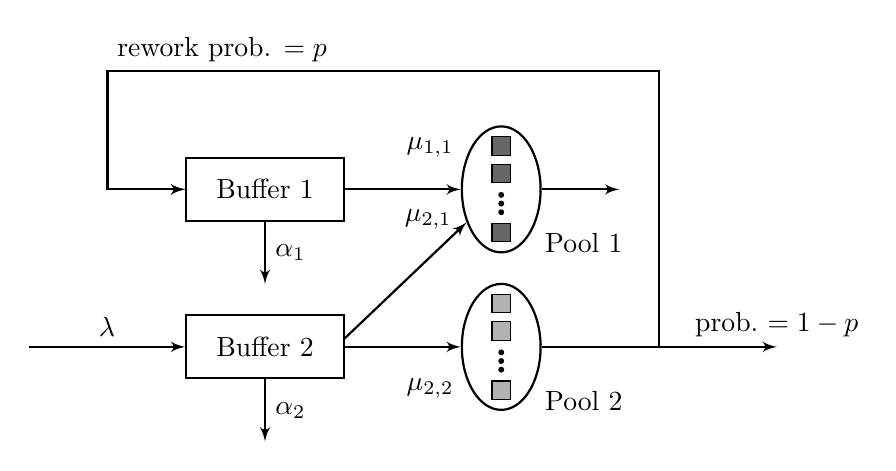
\begin{tikzpicture}[auto, >=latex']
    \everymath{\displaystyle}
    \tikzstyle{every picture}+=[remember picture]

    \tikzstyle{coor-format} = [coordinate]
    \tikzstyle{b-format} = [draw=black, thick,
                            minimum height=0.8cm, minimum width=2cm]
    \tikzstyle{s1-format} = [rectangle, draw=black, fill=black!60]
    \tikzstyle{s2-format} = [rectangle, draw=black, fill=black!30]
    \tikzstyle{p-format} = [ellipse, draw=black, thick,
                            minimum height=1.6cm, minimum width=1cm]

    \node [coor-format] (In1) {};
    \node [b-format, right of=In1, node distance=2cm] (Buf1) {Buffer 1};
    \draw [draw,->, thick] (In1) -- (Buf1);

    \node [coor-format, below of=Buf1, node distance=1.2cm] (Abd1) {};
    \draw [draw,->, thick] (Buf1) -- node {$\alpha_1$} (Abd1);

    \node [p-format, right of=Buf1, node distance=3cm, label=-45:Pool 1,
           label=150:{$\mu_{1,1}$}, label=-165:{$\mu_{2,1}$}] (Pool1) {};
    \draw [draw,->, thick] (Buf1) -- (Pool1);

    \node [coor-format, right of=Pool1, node distance=1.5cm] (Out1) {};
    \draw [draw,->, thick] (Pool1) -- (Out1);

    \node [coor-format,below of = In1, node distance = 2cm] (In2) {};
    \node [b-format, right of=In2, node distance=2cm] (Buf2) {Buffer 2};
    \draw [draw,->, thick] (In2)+(-1cm,0) --node {$\lambda$} (Buf2);

    \node [p-format, right of=Buf2, node distance=3cm,
           label=-45:Pool 2,label=-150:$\mu_{2,2}$] (Pool2) {};
    \draw [draw,->, thick] (Buf2) -- (Pool2);
    \draw [draw,->, thick] (Buf2.east)+(-0.01cm,0.1cm) -- (Pool1);

    \node [coor-format, below of=Buf2, node distance=1.2cm] (Abd2) {};
    \draw [draw,->, thick] (Buf2) -- node {$\alpha_2$} (Abd2);

    \node [coor-format, right of=Pool2, node distance=3.5cm,
    label=90:{prob.\ $=1-p$}] (Out2) {};
    \draw [draw,->, thick] (Pool2) -- (Out2);

    \node [coor-format, above of = In1,
           node distance=1.5cm, label=45:rework prob. {$=p$}](upper-left){};
    \path [draw, -, thick] (Out2)+(-1.5cm,0) |- (upper-left);

    \draw [draw, ->, thick] (upper-left)+(0,0.014cm) |- (Buf1);

    \node at (5cm,0.55cm) [s1-format]{};
    \node at (5cm,0.2cm) [s1-format]{};
    \draw [draw=black, fill=black]
           (5cm,-0.07cm) circle (0.03cm);
    \draw [draw=black, fill=black]
           (5cm,-0.18cm) circle (0.03cm);
    \draw [draw=black, fill=black]
           (5cm,-0.29cm) circle (0.03cm);
    \node at (5cm,-0.55cm) [s1-format]{};

    \node at (5cm,0.55cm-2cm) [s2-format]{};
    \node at (5cm,0.2cm-2cm) [s2-format]{};
    \draw [draw=black, fill=black]
           (5cm,-0.07cm-2cm) circle (0.03cm);
    \draw [draw=black, fill=black]
           (5cm,-0.18cm-2cm) circle (0.03cm);
    \draw [draw=black, fill=black]
           (5cm,-0.29cm-2cm) circle (0.03cm);
    \node at (5cm,-0.55cm-2cm) [s2-format]{};
\end{tikzpicture}

  \caption{A schematic Model of Outsourcing with rework}
  \label{fig:N-model-rework}
\end{figure}

% Project-specific figures
\begin{figure}[htbp]
  \centering
  \begin{tikzpicture}
  \definecolor{color0}{rgb}{0.12156862745098,0.466666666666667,0.705882352941177}

  \begin{axis}[
  axis line style={white!15!black},
  tick align=outside,
  tick pos=left,
  x grid style={white!80!black},
  xmin=50, xmax=190,
  xlabel={Dimension},
  ylabel={Cumulative Regret},
  xtick style={color=white!15!black},
  y grid style={white!80!black},
  ymin=550, ymax=1100,
  ytick style={color=white!15!black},
  width=15cm, height = 8cm
  ]
  \addplot [semithick, color0]
  table {%
  50 552.948441141061
  60 561.458791200929
  70 601.185083349932
  80 656.624488332352
  90 588.205612553125
  100 584.694727360938
  110 689.972024228008
  120 673.722985179478
  130 642.992142072734
  140 754.5337634725
  150 764.145987873789
  160 842.91479035342
  170 822.626056821395
  180 903.667888222128
  190 1070.22626013285
  };
  \end{axis}
\end{tikzpicture}

  \caption{Gaussian Mechanism + Lasso Bandits}
  \label{fig:Gaussian+Lasso}
\end{figure}

\begin{figure}[htbp]
  \centering
  % Contains subfigures - use inside a figure environment
\begin{subfigure}{\textwidth}
  \centering
  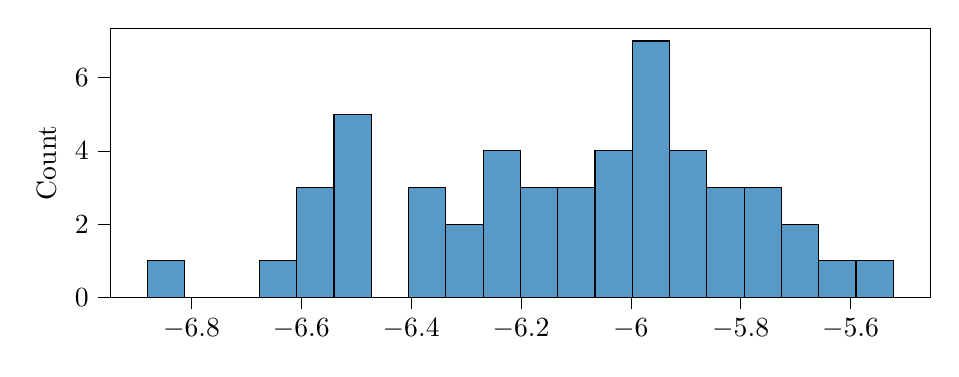
\begin{tikzpicture}
    \definecolor{color0}{rgb}{0.12156862745098,0.466666666666667,0.705882352941177}
    \begin{axis}[
    tick align=outside,
    tick pos=left,
    x grid style={white!69.0196078431373!black},
    xmin=-6.94795252966014, xmax=-5.45416511327468,
    xtick style={color=black},
    y grid style={white!69.0196078431373!black},
    ylabel={Count},
    ymin=0, ymax=7.35,
    ytick style={color=black},
    width=12cm, height=5cm
    ]
    \draw[draw=black,fill=color0,fill opacity=0.75] (axis cs:-6.88005310164262,0) rectangle (axis cs:-6.8121536736251,1);
    \draw[draw=black,fill=color0,fill opacity=0.75] (axis cs:-6.8121536736251,0) rectangle (axis cs:-6.74425424560758,0);
    \draw[draw=black,fill=color0,fill opacity=0.75] (axis cs:-6.74425424560758,0) rectangle (axis cs:-6.67635481759006,0);
    \draw[draw=black,fill=color0,fill opacity=0.75] (axis cs:-6.67635481759006,0) rectangle (axis cs:-6.60845538957254,1);
    \draw[draw=black,fill=color0,fill opacity=0.75] (axis cs:-6.60845538957254,0) rectangle (axis cs:-6.54055596155502,3);
    \draw[draw=black,fill=color0,fill opacity=0.75] (axis cs:-6.54055596155502,0) rectangle (axis cs:-6.4726565335375,5);
    \draw[draw=black,fill=color0,fill opacity=0.75] (axis cs:-6.4726565335375,0) rectangle (axis cs:-6.40475710551998,0);
    \draw[draw=black,fill=color0,fill opacity=0.75] (axis cs:-6.40475710551998,0) rectangle (axis cs:-6.33685767750246,3);
    \draw[draw=black,fill=color0,fill opacity=0.75] (axis cs:-6.33685767750246,0) rectangle (axis cs:-6.26895824948493,2);
    \draw[draw=black,fill=color0,fill opacity=0.75] (axis cs:-6.26895824948493,0) rectangle (axis cs:-6.20105882146741,4);
    \draw[draw=black,fill=color0,fill opacity=0.75] (axis cs:-6.20105882146741,0) rectangle (axis cs:-6.13315939344989,3);
    \draw[draw=black,fill=color0,fill opacity=0.75] (axis cs:-6.13315939344989,0) rectangle (axis cs:-6.06525996543237,3);
    \draw[draw=black,fill=color0,fill opacity=0.75] (axis cs:-6.06525996543237,0) rectangle (axis cs:-5.99736053741485,4);
    \draw[draw=black,fill=color0,fill opacity=0.75] (axis cs:-5.99736053741485,0) rectangle (axis cs:-5.92946110939733,7);
    \draw[draw=black,fill=color0,fill opacity=0.75] (axis cs:-5.92946110939733,0) rectangle (axis cs:-5.86156168137981,4);
    \draw[draw=black,fill=color0,fill opacity=0.75] (axis cs:-5.86156168137981,0) rectangle (axis cs:-5.79366225336229,3);
    \draw[draw=black,fill=color0,fill opacity=0.75] (axis cs:-5.79366225336229,0) rectangle (axis cs:-5.72576282534477,3);
    \draw[draw=black,fill=color0,fill opacity=0.75] (axis cs:-5.72576282534477,0) rectangle (axis cs:-5.65786339732725,2);
    \draw[draw=black,fill=color0,fill opacity=0.75] (axis cs:-5.65786339732725,0) rectangle (axis cs:-5.58996396930973,1);
    \draw[draw=black,fill=color0,fill opacity=0.75] (axis cs:-5.58996396930973,0) rectangle (axis cs:-5.52206454129221,1);
    \end{axis}
  \end{tikzpicture}
  \caption{Dimension $d=50$}
\end{subfigure}
\begin{subfigure}{\textwidth}
  \centering
  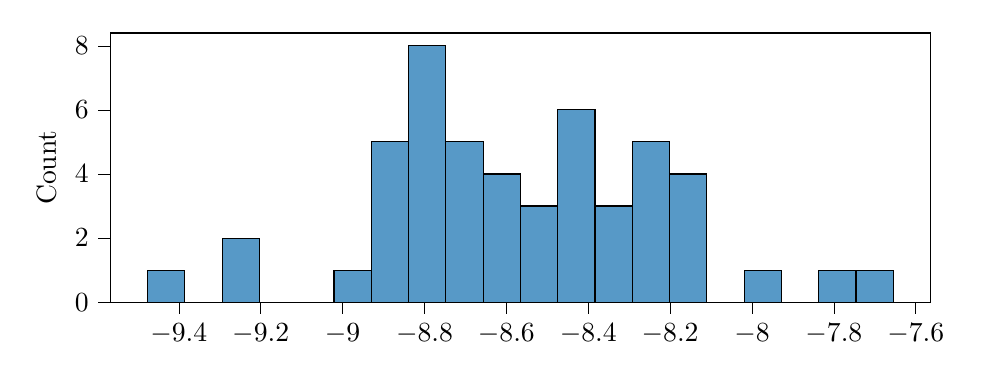
\begin{tikzpicture}
    \definecolor{color0}{rgb}{0.12156862745098,0.466666666666667,0.705882352941177}
    \begin{axis}[
    tick align=outside,
    tick pos=left,
    x grid style={white!69.0196078431373!black},
    xmin=-9.56749670360284, xmax=-7.56375481022318,
    xtick style={color=black},
    y grid style={white!69.0196078431373!black},
    ylabel={Count},
    ymin=0, ymax=8.4,
    ytick style={color=black},
    width=12cm, height=5cm
    ]
    \draw[draw=black,fill=color0,fill opacity=0.75] (axis cs:-9.47641752663104,0) rectangle (axis cs:-9.38533834965923,1);
    \draw[draw=black,fill=color0,fill opacity=0.75] (axis cs:-9.38533834965923,0) rectangle (axis cs:-9.29425917268743,0);
    \draw[draw=black,fill=color0,fill opacity=0.75] (axis cs:-9.29425917268743,0) rectangle (axis cs:-9.20317999571563,2);
    \draw[draw=black,fill=color0,fill opacity=0.75] (axis cs:-9.20317999571563,0) rectangle (axis cs:-9.11210081874383,0);
    \draw[draw=black,fill=color0,fill opacity=0.75] (axis cs:-9.11210081874383,0) rectangle (axis cs:-9.02102164177203,0);
    \draw[draw=black,fill=color0,fill opacity=0.75] (axis cs:-9.02102164177203,0) rectangle (axis cs:-8.92994246480022,1);
    \draw[draw=black,fill=color0,fill opacity=0.75] (axis cs:-8.92994246480022,0) rectangle (axis cs:-8.83886328782842,5);
    \draw[draw=black,fill=color0,fill opacity=0.75] (axis cs:-8.83886328782842,0) rectangle (axis cs:-8.74778411085662,8);
    \draw[draw=black,fill=color0,fill opacity=0.75] (axis cs:-8.74778411085662,0) rectangle (axis cs:-8.65670493388481,5);
    \draw[draw=black,fill=color0,fill opacity=0.75] (axis cs:-8.65670493388481,0) rectangle (axis cs:-8.56562575691301,4);
    \draw[draw=black,fill=color0,fill opacity=0.75] (axis cs:-8.56562575691301,0) rectangle (axis cs:-8.47454657994121,3);
    \draw[draw=black,fill=color0,fill opacity=0.75] (axis cs:-8.47454657994121,0) rectangle (axis cs:-8.38346740296941,6);
    \draw[draw=black,fill=color0,fill opacity=0.75] (axis cs:-8.38346740296941,0) rectangle (axis cs:-8.2923882259976,3);
    \draw[draw=black,fill=color0,fill opacity=0.75] (axis cs:-8.2923882259976,0) rectangle (axis cs:-8.2013090490258,5);
    \draw[draw=black,fill=color0,fill opacity=0.75] (axis cs:-8.2013090490258,0) rectangle (axis cs:-8.110229872054,4);
    \draw[draw=black,fill=color0,fill opacity=0.75] (axis cs:-8.110229872054,0) rectangle (axis cs:-8.0191506950822,0);
    \draw[draw=black,fill=color0,fill opacity=0.75] (axis cs:-8.0191506950822,0) rectangle (axis cs:-7.92807151811039,1);
    \draw[draw=black,fill=color0,fill opacity=0.75] (axis cs:-7.92807151811039,0) rectangle (axis cs:-7.83699234113859,0);
    \draw[draw=black,fill=color0,fill opacity=0.75] (axis cs:-7.83699234113859,0) rectangle (axis cs:-7.74591316416679,1);
    \draw[draw=black,fill=color0,fill opacity=0.75] (axis cs:-7.74591316416679,0) rectangle (axis cs:-7.65483398719499,1);
    \end{axis}
  \end{tikzpicture}
  \caption{Dimension $d=100$}
\end{subfigure}
\begin{subfigure}{\textwidth}
  \centering
  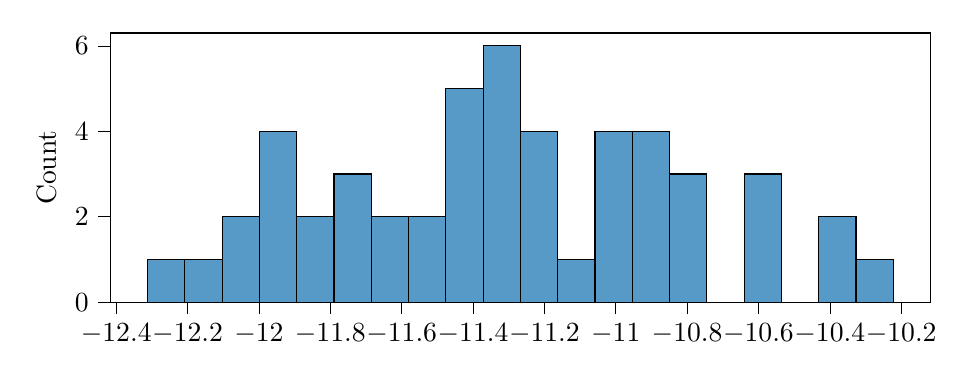
\begin{tikzpicture}
    \definecolor{color0}{rgb}{0.12156862745098,0.466666666666667,0.705882352941177}
    \begin{axis}[
    tick align=outside,
    tick pos=left,
    x grid style={white!69.0196078431373!black},
    xmin=-12.4168122668345, xmax=-10.11762550417,
    xtick style={color=black},
    y grid style={white!69.0196078431373!black},
    ylabel={Count},
    ymin=0, ymax=6.3,
    ytick style={color=black},
    width=12cm, height=5cm
    ]
    \draw[draw=black,fill=color0,fill opacity=0.75] (axis cs:-12.3123037776225,0) rectangle (axis cs:-12.2077952884105,1);
    \draw[draw=black,fill=color0,fill opacity=0.75] (axis cs:-12.2077952884105,0) rectangle (axis cs:-12.1032867991984,1);
    \draw[draw=black,fill=color0,fill opacity=0.75] (axis cs:-12.1032867991984,0) rectangle (axis cs:-11.9987783099864,2);
    \draw[draw=black,fill=color0,fill opacity=0.75] (axis cs:-11.9987783099864,0) rectangle (axis cs:-11.8942698207744,4);
    \draw[draw=black,fill=color0,fill opacity=0.75] (axis cs:-11.8942698207744,0) rectangle (axis cs:-11.7897613315624,2);
    \draw[draw=black,fill=color0,fill opacity=0.75] (axis cs:-11.7897613315624,0) rectangle (axis cs:-11.6852528423503,3);
    \draw[draw=black,fill=color0,fill opacity=0.75] (axis cs:-11.6852528423503,0) rectangle (axis cs:-11.5807443531383,2);
    \draw[draw=black,fill=color0,fill opacity=0.75] (axis cs:-11.5807443531383,0) rectangle (axis cs:-11.4762358639263,2);
    \draw[draw=black,fill=color0,fill opacity=0.75] (axis cs:-11.4762358639263,0) rectangle (axis cs:-11.3717273747143,5);
    \draw[draw=black,fill=color0,fill opacity=0.75] (axis cs:-11.3717273747143,0) rectangle (axis cs:-11.2672188855022,6);
    \draw[draw=black,fill=color0,fill opacity=0.75] (axis cs:-11.2672188855022,0) rectangle (axis cs:-11.1627103962902,4);
    \draw[draw=black,fill=color0,fill opacity=0.75] (axis cs:-11.1627103962902,0) rectangle (axis cs:-11.0582019070782,1);
    \draw[draw=black,fill=color0,fill opacity=0.75] (axis cs:-11.0582019070782,0) rectangle (axis cs:-10.9536934178662,4);
    \draw[draw=black,fill=color0,fill opacity=0.75] (axis cs:-10.9536934178662,0) rectangle (axis cs:-10.8491849286541,4);
    \draw[draw=black,fill=color0,fill opacity=0.75] (axis cs:-10.8491849286541,0) rectangle (axis cs:-10.7446764394421,3);
    \draw[draw=black,fill=color0,fill opacity=0.75] (axis cs:-10.7446764394421,0) rectangle (axis cs:-10.6401679502301,0);
    \draw[draw=black,fill=color0,fill opacity=0.75] (axis cs:-10.6401679502301,0) rectangle (axis cs:-10.5356594610181,3);
    \draw[draw=black,fill=color0,fill opacity=0.75] (axis cs:-10.5356594610181,0) rectangle (axis cs:-10.431150971806,0);
    \draw[draw=black,fill=color0,fill opacity=0.75] (axis cs:-10.431150971806,0) rectangle (axis cs:-10.326642482594,2);
    \draw[draw=black,fill=color0,fill opacity=0.75] (axis cs:-10.326642482594,0) rectangle (axis cs:-10.222133993382,1);
    \end{axis}
  \end{tikzpicture}
  \caption{Dimension $d=200$}
\end{subfigure}

  \caption{Simulation Study for Bandit Inference}
  \label{fig:estimator}
\end{figure}


% ==================== REFERENCES ====================
\newpage

\setcounter{page}{1}
\pagenumbering{arabic}
\setlength{\bibsep}{3pt plus 6pt}
\begin{spacing}{1.42}
\bibliography{ref}
\end{spacing}
\newpage


% ==================== Gantt Chart ======================

\section*{Gantt Chart}
\addcontentsline{toc}{section}{Gantt Chart}

\pagestyle{empty}
\setcounter{page}{1}
\pagenumbering{roman}

%
% A fairly complicated example from section 2.9 of the package
% documentation. This reproduces an example from Wikipedia:
% http://en.wikipedia.org/wiki/Gantt_chart
%
{
\definecolor{barblue}{RGB}{153,204,254}
\definecolor{groupblue}{RGB}{51,102,254}
\definecolor{linkred}{RGB}{165,0,33}
\renewcommand\sfdefault{phv}
\renewcommand\mddefault{mc}
\renewcommand\bfdefault{bc}
\setganttlinklabel{s-s}{START-TO-START}
\setganttlinklabel{f-s}{FINISH-TO-START}
\setganttlinklabel{f-f}{FINISH-TO-FINISH}
\sffamily
\begin{adjustbox}{width=\textwidth,center}
\begin{ganttchart}[
    canvas/.append style={fill=none, draw=black!5, line width=.75pt},
    hgrid style/.style={draw=black!5, line width=.75pt},
    vgrid={*1{draw=black!5, line width=.75pt}},
    title/.style={draw=none, fill=none},
    title label font=\bfseries\footnotesize,
    title label node/.append style={below=0pt},
    include title in canvas=false,
    bar label font=\mdseries\small\color{black!70},
    bar label node/.append style={left=1cm},
    bar/.append style={draw=none, fill=barblue},
    bar incomplete/.append style={fill=barblue},
    bar progress label font=\mdseries\footnotesize\color{black!70},
    group/.append style={fill=groupblue},
    group incomplete/.append style={fill=groupblue},
    group left shift=0,
    group right shift=0,
    group height=.5,
    group peaks tip position=0,
    group label node/.append style={left=0.6cm},
    group progress label font=\bfseries\small,
  ]{1}{18}
  \gantttitle[
    title label node/.append style={below left=12pt and -12pt}
    ]{Year 1}{6}
  \gantttitle[
    title label node/.append style={below left=12pt and -10pt}
    ]{Year 2}{6}
  \gantttitle[
    title label node/.append style={below left=12pt and -10pt}
    ]{Year 3}{6}\\
  \gantttitlelist{1,3,5,7,9,11,13,15,17,19,21,23,25,27,29,31,33,35}{1} \\
  \ganttgroup{High Dimensional Bandits with DP}{1}{11} \\
  \ganttbar{Formulate the problem}{1}{1} \\
  \ganttbar[
    name=WBS1A
  ]{Design private estimator in linear model}{2}{4} \\
  \ganttbar[
    name=WBS1B
  ]{Design private estimator in GLM}{4}{6} \\
  \ganttbar[
    name=WBS1C
  ]{Analyze regret incurred using above estimator}{6}{8} \\
  \ganttbar[
    name=WBS1C
  ]{Derive computational efficient variant}{9}{11} \\
  [grid]
  \ganttgroup[]{Inference on High Dimensional DP Bandit Data}{9}{18} \\
  \ganttbar[]{Formulate High Dimensional Bandits with DP}{9}{10}\\
  \ganttbar[]{Developing bias bounds for the lasso estimator}{10}{13} \\
  \ganttbar[]{Design debias procedure}{13}{15}\\
  \ganttbar[]{Derive computational efficient variant}{15}{18}
\end{ganttchart}
\end{adjustbox}
}

\newpage

% ==================== EDUCATION PLAN ====================

\section*{Education Plan}
\addcontentsline{toc}{section}{Education Plan}
\pagestyle{empty}
\begin{spacing}{1.32}

This research project will generate new insights, both quantitatively and qualitatively, into the design and implementation of novel machine learning algorithms on data privacy in high dimensional decision-making setting. Despite the increasing use and importance of these issues in machine learning and data technology, few courses currently focus on this emerging area.
We plan to turn the insights and domain knowledge gained from this project into relevant course materials for undergraduate, graduate, and professional education.
The material generated from this project can be taught with different focuses at various levels.

At my university, I have developed a series of courses, \emph{IEDA 2520 Probability}, \emph{IEDA 2540 Statistics} and \emph{IEDA 3650  predictive analytics}, which has been well received by students.
In particular, IEDA 3650 focuses on various machine learning algorithms.
Based on some of the resulting outcomes, we plan to involve the course into incorporate privacy and bandit algorithms.
Since our proposed research comes from practical applications, some of the results will become perfect material for the case study of the proposed new course.
For teaching undergraduate students, the key is to make the basic elements clear and illustrate a few simplified models without losing the essence, such as the fundamental principle of privacy protection. By contrast, Ph.D.\ level courses will focus on the theoretical analysis of various privacy mechanisms and the related algorithms.
In addition to developing undergraduate courses, I also plan to incorporate some methodologies developed in this research into the course \emph{IEDA 6000E Advanced Methods in Machine Learning} targeted for Ph.D. students in our field by focusing more on the theoretical aspects.
It is also possible to contribute to the department core Ph.D.\ course \emph{IEDA 5270 Engineering Statistics and Data Analytics}.
The purpose is to strengthen the training of students (both undergraduate and postgraduate) by improving students' analytical and logical thinking ability, and problem-solving skills for real-world applications.

In addition to fostering the integration of research and education by developing course materials, this research will also involve research students (both undergraduate and Ph.D.\ students with strong mathematical and programming skills) in numerical experiments because code implementation and simulation are an integral part of the project.
The proposed research has the potential to be rich enough to cover several Ph.D.\ dissertations.
In fact, we have already involved two Ph.D.\ students in a preliminary study, including a literature review and basic model analysis.
Students who participate in this research will gain valuable insight into the intricacies underlying mathematics. This research project will help grow future academic and industry leaders.

\end{spacing}

\end{document}
